\section{Library Language}
The Domain Specific Language (DSL) we have created is an attempt at modelling a Library system. We have a chosen the context of a public library as opposed to a specialised facility such as a university or law library. The DSL is naturally constrained by our development tool and as such  is comprised of three main entities: Objects, Relationships and Roles. These entities are described in the following sections. 

\subsection{Objects}
Objects represent physical entities such as loanable items, library equipment and people such as library users and employees. Examples of Objects within the system include a book shown in Figure~\ref{fig:objbook}, people such as Author shown in 

\begin{figure}
  \centering
  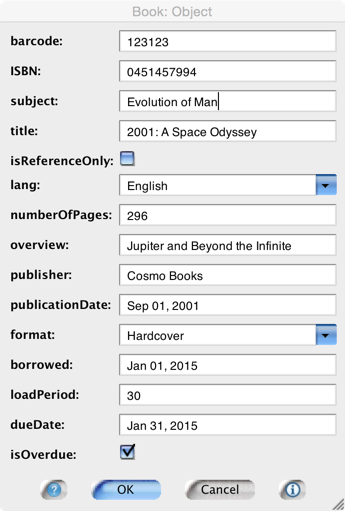
\includegraphics[width=0.5\textwidth]{obj_book}  
  \caption{A book object from the DSL.}
  \label{fig:objbook}
\end{figure}

\begin{figure}
  \centering
  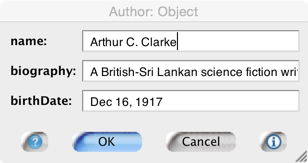
\includegraphics[width=0.5\textwidth]{obj_author}
  \caption{A book object from the DSL.}
  \label{fig:objbook}
\end{figure}

\begin{figure}
  \centering
  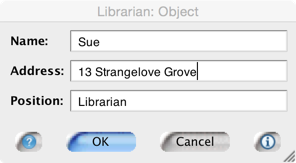
\includegraphics[width=0.5\textwidth]{obj_librarian}
  \caption{A book object from the DSL.}
  \label{fig:objbook}
\end{figure}

\begin{figure}
  \centering
  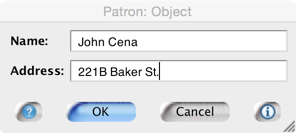
\includegraphics[width=0.5\textwidth]{obj_patron}
  \caption{A book object from the DSL.}
  \label{fig:objbook}
\end{figure}







\subsection{Relationships}
Relationships describe methods by which objects within the DSL may interact.
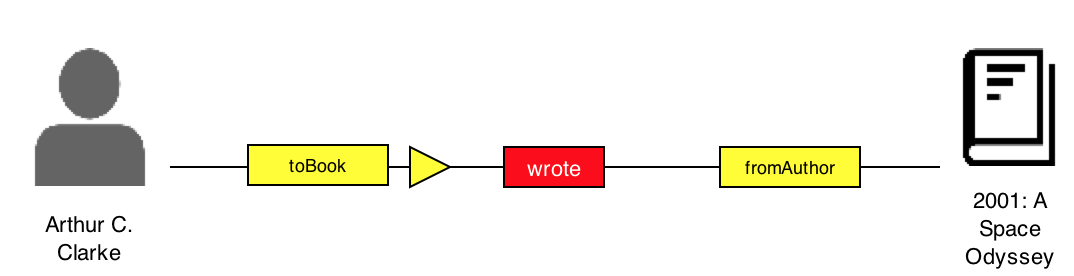
\includegraphics[width=0.5\textwidth]{rel_wrote}
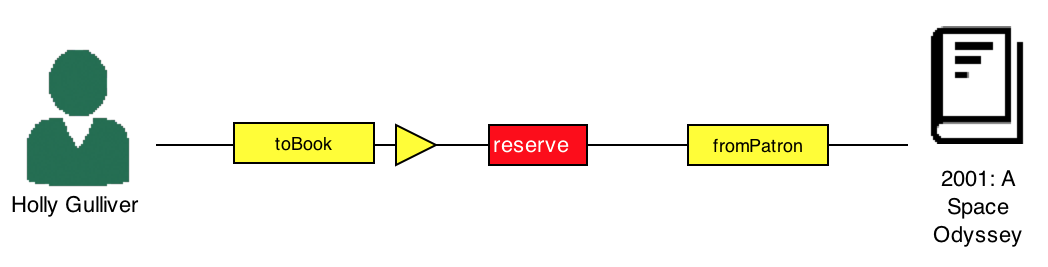
\includegraphics[width=0.5\textwidth]{rel_reserve}
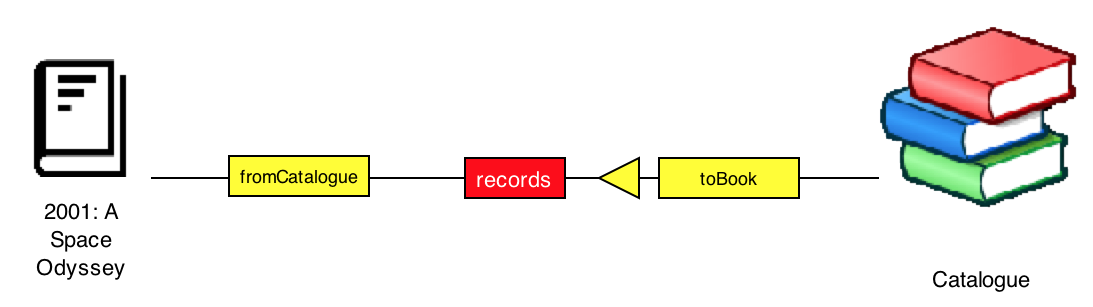
\includegraphics[width=0.5\textwidth]{rel_records}


\subsection{Roles}
 Roles define constraints on the types of objects that may mutually INHABIT? TAKE THE PLACE IN THE RELATIONSHIP, ?BE?, ?RESIDE? word please  end of a relationship between those objects. 


\subsection{Constraints}
 Additionally constraints may be defined surrounding the semantics of relationships. These constraints fall into four categories:
Connectivity: cardinality and type of some shit about the thing with a thing. 
Occurrence: constraint surrounding the number of a unique objects may appear in a graph
Uniqueness: uniqueness constraints for property values such as ID etc
Port: No fucking idea what the shit port was for, probably something to do with ships.
Creating and applying constraints allows further development and enrichment of DSL semantics.  
\subsection{Objects}


